\chapter{Method}
\label{cap:Method}

In this chapter, the method used to conduct this Master thesis will be described. The entire method is broken down into several sub processes to better structure and describe, as illustrated in  \ref{fig:Method_process}.  

\begin{figure}[H]
    \centering
    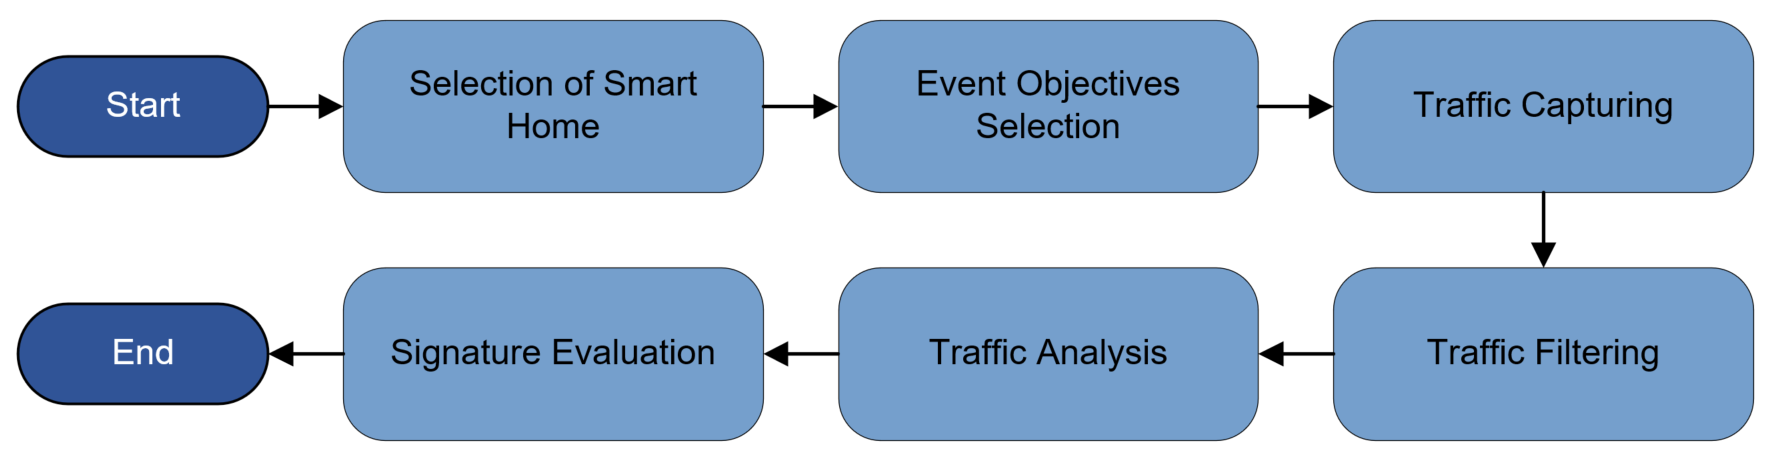
\includegraphics[width=\textwidth]{figures/Method_process.png}
    \caption{Overall Method process}
    \label{fig:Method_process}
\end{figure}



\section{Device and Environment Selection}
Due to limited resources of this project it is important to find the best satiable device for this research. Since all the testing and analysis is based on the data generated by the robot vacuum cleaner, it will be selected first. To ensure that the thesis is relevant, there will be conducted a robot vacuum cleaner survey to find the most relevant model.

\subsection{Selection of Robot Vacuum Cleaner Model}
First there will be defined some specification needed on a robot vacuum cleaner to be selected. The research will have the largest scientific contribution if the vacuum cleaner is selected based on the specifications listed below.
\begin{itemize}
    \item Communication protocol: Wi-Fi is the most wide spread communication protocol in today's smart homes \cite{robotsel1}. Eavesdropping devices and analysis tools are also available for IEEE.802.11 and network layers higher in the OSI model \cite{osimodel}. The selected robot vacuum cleaner therefore need to use wi-fi as a primary communication protocol.
    
    \item Smart Home Features; The robot vacuum cleaner needs to have several different smart home features. As more features available the more attribution and potential information can be exposed. The number of different smart home features will increase the communication with the could services for the selected model \cite{robotsel4}.
    
    \item Popularity; The prevalence of different vendors and models will vary, based on the number of sold and used devices. Overall usage will increase the relevance and, the scientific contribution of this research.  
\end{itemize}

Data and ratings from these three robot vacuum cleaner review sites \cite{robotsel11}\cite{robotsel12}\cite{robotsel13}, was used  as the first phase of the selection. The summary of all these reviews will be used to determine most reliable robot vacuum cleaner vendors. To determine the popularity of the different vendors, statistics about downloads and ratings is gathered from Google Play \cite{GooglePlay}.

\subsection{Result Selection Robot Vacuum Cleaner}

Results from the review sites shows that the two best robot vaccum cleaner vendors is, Irobot and Roborock. This results are presented in  Table \ref{tab:Robotreviewsites}

\begin{table}[H]
    \label{tab:Robotreviewsites}
    \centering
    \begin{subtable}[b]{0.45\linewidth}
        \centering
        \caption{Results from review-site \cite{robotsel11}}
        \begin{tabular}{|l|l|}
            \hline 
            \textbf{Vendor} & \textbf{Number on top ten} \\ \hline
            Irobot      & 3                 \\                   \hline
            Roborock    & 3                 \\                   \hline
            Neatsvor    & 0                 \\                   \hline
            Ecovacs     & 0                 \\                   \hline
            iLife       & 2                 \\                   \hline
        \end{tabular}
    \end{subtable}
    \hspace{0.5cm}
    \begin{subtable}[b]{0.45\linewidth}
        \centering
        \caption{Results from review-site \cite{robotsel12}}
        \begin{tabular}{|l|l|}
            \hline
            \textbf{Vendor}    & \textbf{Number on top ten} \\ \hline
            Irobot      & 2                 \\                   \hline
            Roborock    & 2                 \\                   \hline
            Neatsvor    & 0                 \\                   \hline
            Ecovacs     & 2                 \\                   \hline
            iLife       & 1                 \\                   \hline
        \end{tabular}
    \end{subtable}
    \begin{subtable}[b]{0.45\linewidth}
        \centering
        \caption{Results from review-site \cite{robotsel13}}
        \begin{tabular}{|l|l|}
            \hline
            \textbf{Vendor}    & \textbf{Number on top ten} \\ \hline
            Irobot      & 2                 \\                   \hline
            Roborock    & 2                 \\                   \hline
            Neatsvor    & 3                 \\                   \hline
            Ecovacs     & 1                 \\                   \hline
            iLife       & 0                 \\                   \hline
        \end{tabular}
    \end{subtable}
    \hspace{0.5cm}
    \begin{subtable}[b]{0.45\linewidth}
        \centering
        \caption{Summary of all review-sites}
        \begin{tabular}{|l|l|}
            \hline
            \textbf{Vendor}    & \textbf{Number on top ten} \\ \hline
            Irobot      & 7                 \\                   \hline
            Roborock    & 7                 \\                   \hline
            Neatsvor    & 3                 \\                   \hline
            Ecovacs     & 3                 \\                   \hline
            iLife       & 3                 \\                   \hline
        \end{tabular}
    \end{subtable}
    \caption{Robot vacuum selection review-site}
\end{table}

Applications for different vendors' robot vacuum cleaners are presented in Table \ref{tab:VendorApplicationStat}. It is worth mentioning that the "Smart Life" application are used to control the Neatsvor, but it is a full smart home integration application, not robot vacuum cleaner specific. 

\begin{table}[H]
\centering
\caption{Vendor application statistics}
\label{tab:VendorApplicationStat}
\begin{tabular}{|c|c|c|c|}
\hline
\textbf{Vendor} & \textbf{Application} & \textbf{Downloads} & \textbf{Rating} \\ \hline
Irobot          & Irobot Home          & 5 million +        & 4,0/5,0         \\ \hline
Roborock        & Roborock             & 1 million +        & 4,6/5,0         \\ \hline
Neatsvor        & Smart Life           & 10 million +       & 4,5/5,0         \\ \hline
Ecovacs         & Ecovacs Home         & 1 million +        & 2,5/5,0         \\ \hline
iLife           & iLifehome            & 50 thousand +      & NA              \\ \hline
\end{tabular}
\end{table}
Both Irobot and Roborock received seven recommendations on the review websites. This is significantly higher than the other three vendors on the list, each of which had only three representations. Additionally, both vendors were referenced in all three review sites, which strengthens their credibility. 

In the application download and ratings analysis, the Neatsvor application had over 10 million downloads. However, this application is more focused on smart home integration, and the high number of downloads is likely not solely due to the robot vacuum cleaner. Meanwhile, Evacos home received a 2.5/5.0 rating, and despite having a similar number of downloads as Roborock, it fell short in the selection process. Hence, Irobot and Roborock emerged as the two most relevant vendors. In a comparison of their products, it was found that the Irobot Roomba i7 and Roborock S6 were the best suitable robots according to our requirements \cite{robotsel8} \cite{robotsel6}. The final comparison was conducted using the website \cite{robotsel9}.

Irobot roomba i7 and Roborck S6 have similar reviews and rating all over, and they both have a sufficient number of smart home features required in this research. The fact that the Irobot application is downloaded 5 times more than the Roborock was the decisive factor, and Irobot roomba i7 will be used during this research. 

\subsection{Environment Selection}
The rest of the research environment have to support and allow traffic eavesdropping and analysis, of the Irobot Roomba i7.  Important factors to support in research environment:

\begin{itemize}
    \item IEEE.802.11 WI-FI network
    \item Internet connection
    \item Local wired LAN
    \item Different physical rooms
\end{itemize}

\subsubsection{Physical Environment}
To ensure the validity of the results across diverse settings, the testing will be conducted in two different smart home environments situated in separate cities. The Robot vacuum cleaner will be configured from factory defaults for each smart home environment. Both home environments have independent Internet access, provided by an external Internet Service Provider (ISP). To control the duration of each test, the available are will be restricted to the one room. As the floor space in this room is smaller, the cleaning process will be relatively shorter. An illustration of the two distinct smart home environments is shown in Figure \ref{fig:SmartHomeEnvironments}. These are from now on called Oslo and Drammen.

\begin{figure}[H]
    \centering
    \begin{subfigure}[b]{0.60\textwidth}
        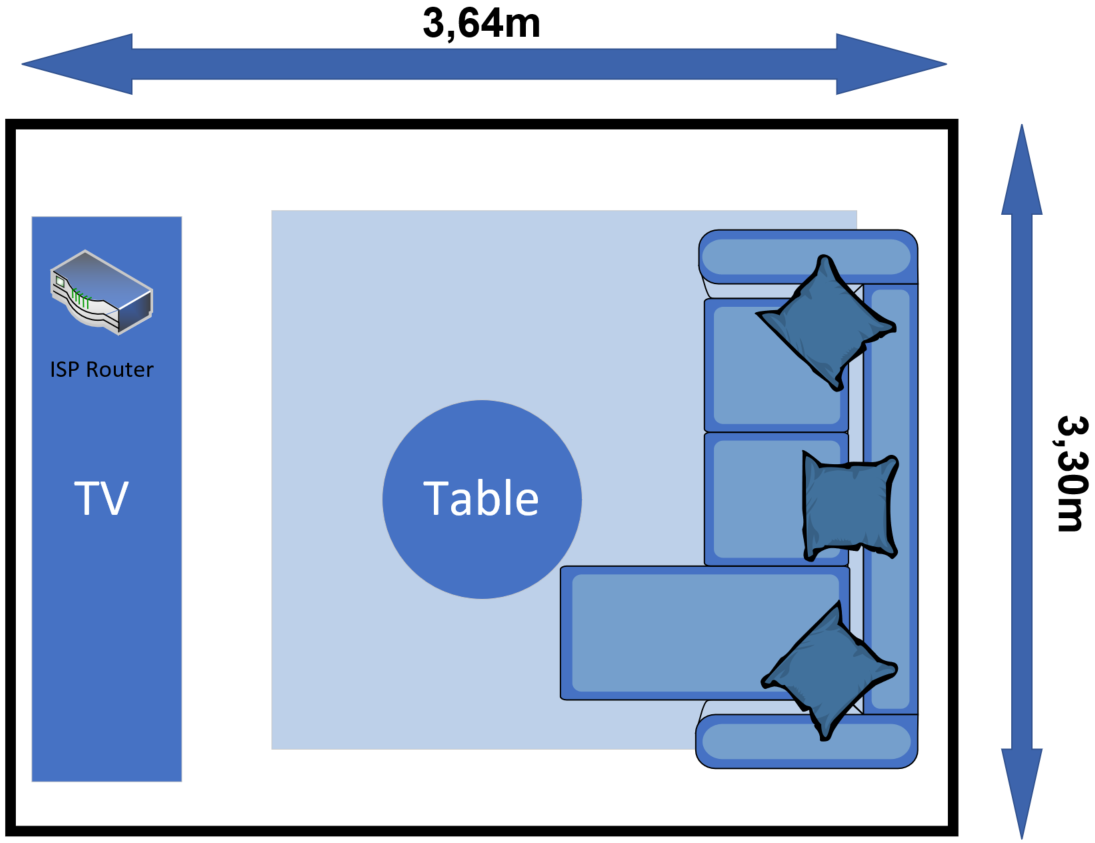
\includegraphics[width=\textwidth]{figures/Environment1.png}
        \caption{The smart home environment in Oslo}
        \label{fig:Environment1}
    \end{subfigure}
    \hfill
    \begin{subfigure}[b]{0.6\textwidth}
        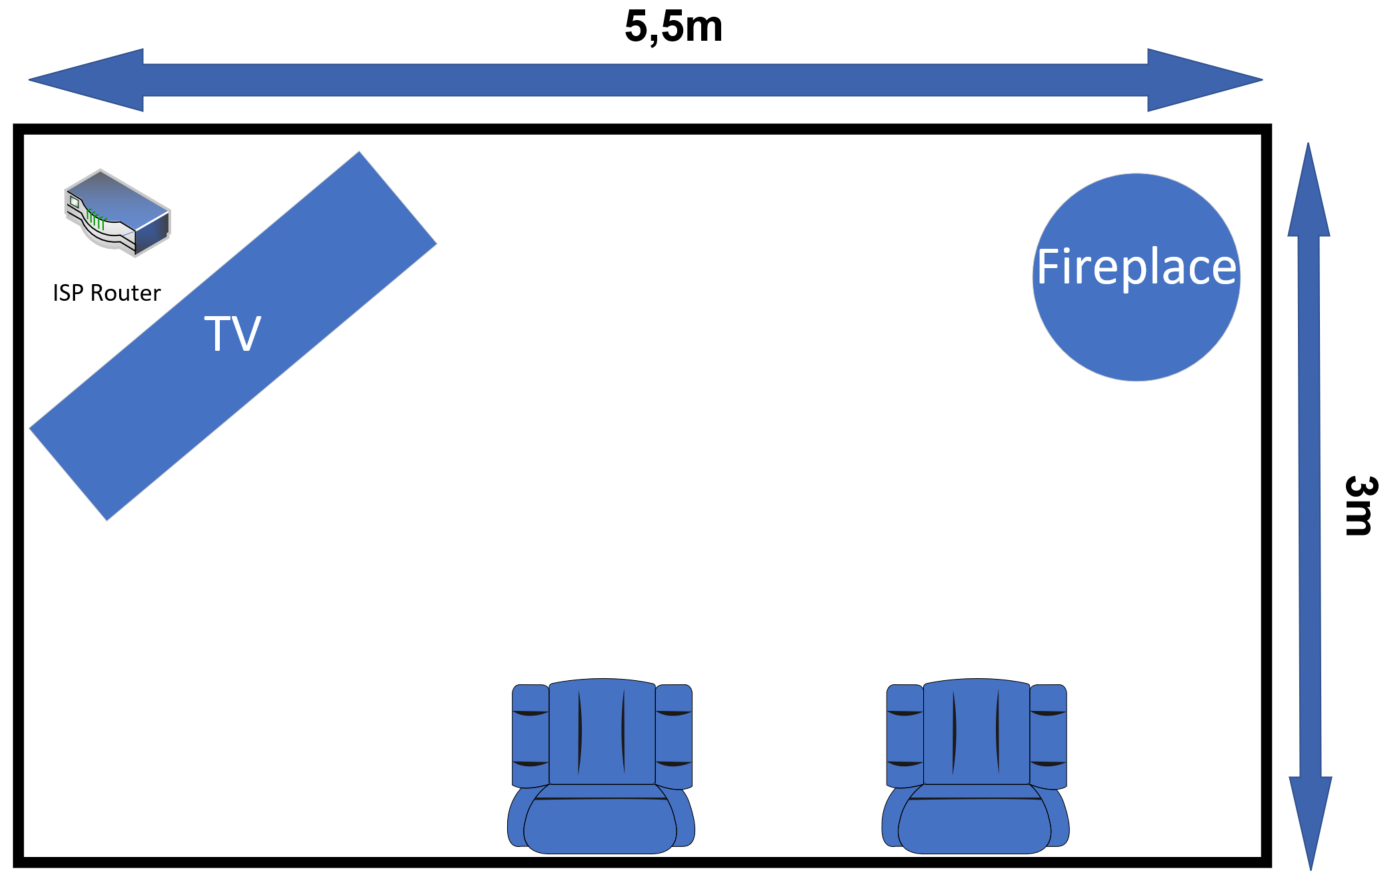
\includegraphics[width=\textwidth]{figures/Environment2.png}
        \caption{The smart home environment in Drammen}
        \label{fig:Environmet2}
    \end{subfigure}
    \caption{The smart home environments used in this thesis}
    \label{fig:SmartHomeEnvironments}
\end{figure}

\subsubsection{Capturing and Analysis Platform}
For the capturing, and analysis platform there are some requirements that needs to be fulfilled.

 The \textit{Capturing platform} needs to be able to operate autonomously, due to continuously capturing of events. It needs software that enables capturing of wireless IEEE.802.11 and wired traffic IEEE.802.3, simultaneously. Tools to transfer the captured data need to be integrated on the selected platform. 
 
 The \textit{Analysis platform} needs to have tools to analysis the traffic, based on the format of the capturing tool. 


As capturing platform the Raspberry PI 3b+ is chosen. This was available through the authors' employer. Kali Linux is selected as the OS, this is a open source operating system, including several different tools to capture and analyse traffic. Dedicated versions are designed for Raspberry PI \cite{kalidownload}. To enable capturing of wireless traffic the wireless network interface card needs to be in \textit{Monitor mode}. For Kali Linux the \textit{TP-LINK TL-WN722N V2/V3} is recommended by \cite{Kali_monitormode_guide}, and is therefore used in this research. 
Analysis platform is a HP Elitebook due to availability. It runs Windows 11 OS which is compatible with several different tools for capturing and analysis.

\subsubsection{Environment Infrastructure}
This research includes eavesdropping of wireless traffic and wired WAN traffic. The two different smart home environments only includes a single ISP router providing both Internet connection and Wi-Fi, and does not have features allowing the capturing platform to eavesdrop the wired traffic generated by the robot vacuum cleaner. Additional infrastructure settings is therefore added below. 
\begin{itemize}
    \item Wireless access point; This access point will create a new SSID only to be used by the Robot vacuum cleaner, this isolates the vacuum cleaner from potential impact from other devices on the WLAN/LAN. The access point will also use Network address translation and translate all traffic to one singe IP address. With this setup, all traffic with the source address of the access point will be either the access point itself, or the robot vacuum cleaner. This will therefore work as a simulated WAN interface, delivered by ISPs
    \item LAN switch; The LAN switch will be directly connected to both the access point and the ISP router. All Internet traffic will therefore be transmitted though the switch. A SPAN port is configured on the switch, this port will monitor all traffic on the port connected to the access point, and duplicate this traffic flow to the port connected to the capturing platform. This setup is illustrated in \ref{fig:WLAN_LAN_setup}
\end{itemize}

\begin{figure}[H]
    \centering
    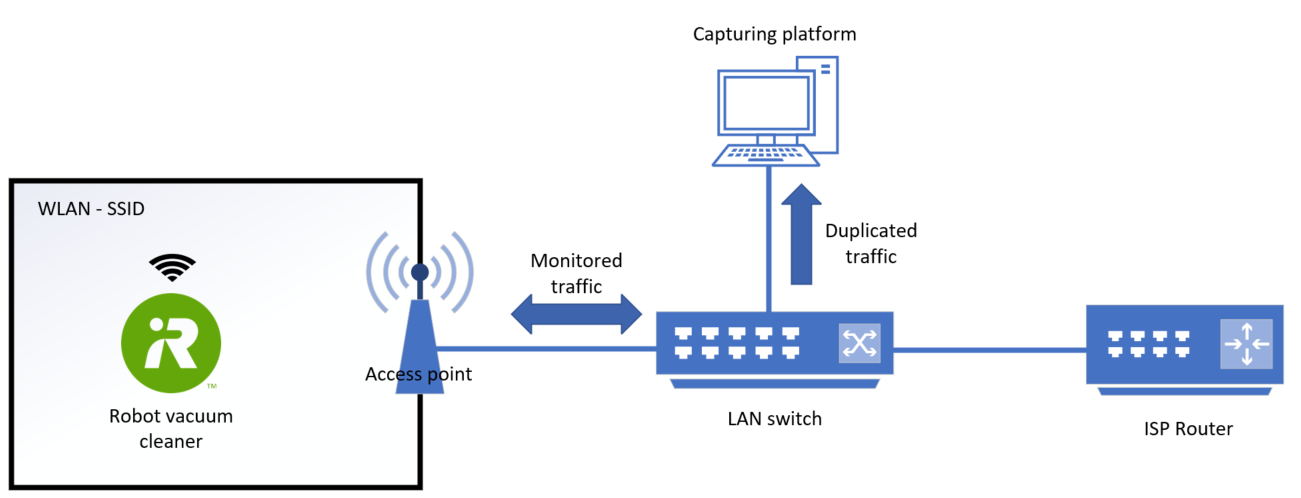
\includegraphics[width=\textwidth]{figures/WLAN_LAN_setup.png}
    \caption{Smart home infrastructure}
    \label{fig:WLAN_LAN_setup}
\end{figure}



\subsubsection{Capturing and Analysis Tools}
Capturing and analysis tools need to be compatible with each other. Stored format from the capturing process needs to be readable in the analysis phase. Tools for these kinds of tasks are many. Whireshark is a widely used network protocol analyser, it allows network capturing and analysis in real-time. It can be used for deep header inspection in all network layers which is not encrypted before the capturing. The application can perform basic identification of a wide range of different protocols across networks layers as well as statistics about the traffic flow. This software is also default installed on Kali Linux OS. Wireshark is also available for Windows on \cite{wireshark_download_2016}.
Tshark is a sub-software included in wireshark and the process which is used to capture traffic on the dedicated network interfaces. This software can be used to capture traffic through CLI. In this process it is possible to define capturing filters which only store traffic that is interesting for the analysis phase. Wireshark is there used in this research.


\section{Traffic Capturing}
This section will describe how the capturing tools are used, and how the overall capturing process is executed. All capturing will be done on the capturing platform, both LAN and WLAN traffic is captured simultaneously. This enables correlation of the traffic for the same event.  

\subsection{Captuing Tools}
Tshark will be used as the capturing tools for both wireless and wired traffic. Two Tshark instances will run simultaneously on the capturing platform. The Tshark filter syntax used for both capturing streams is: 
\\
tshark [ -i <capture interface>|- ] [ -f <capture filter> ] [ -w <outfile>|- ]
\\
The captuing platform has three different NICs:
\begin{itemize}
    \item eth0; is the wired IEEE 802.3 interface which is connected to the SPAN port of the LAN switch.
    \item wlan0; is the buildt in IEEE 802.11 interface on the Raspberry PI.
    \item wlan1; external IEEE 802.11 adapter which is configured to monitor mode.
\end{itemize}

LAN Tshark command:
\\
sudo tshark -i wlan1 -f 'ip.host "WAN address' -w output.pcap
\\
WLAN Tshark command:
\\
sudo tshark -i wlan1 -f 'eth.host "MAC address' -w output.pcap
\\

\subsection{Capturing Process}
The capturing process will be similar for all events, this will create a better foundation to compare the different test results. 
Figure \ref{fig:captuingprocess} illustrate the entire process.
\begin{enumerate}
    \item Star both LAN and WLAN capture, in separate Tshark processes.
    \item Trigger events according to test event matrix. Note event Start and finish. 
    \item If pcap file exceeds 500MB, stop capture, and start new LAN and WLAN capture.
    \item When testing in environment is finished, stop capture. 
    \item Transfer files to analysis platform
\end{enumerate}
   

\begin{figure}[H]
    \centering
    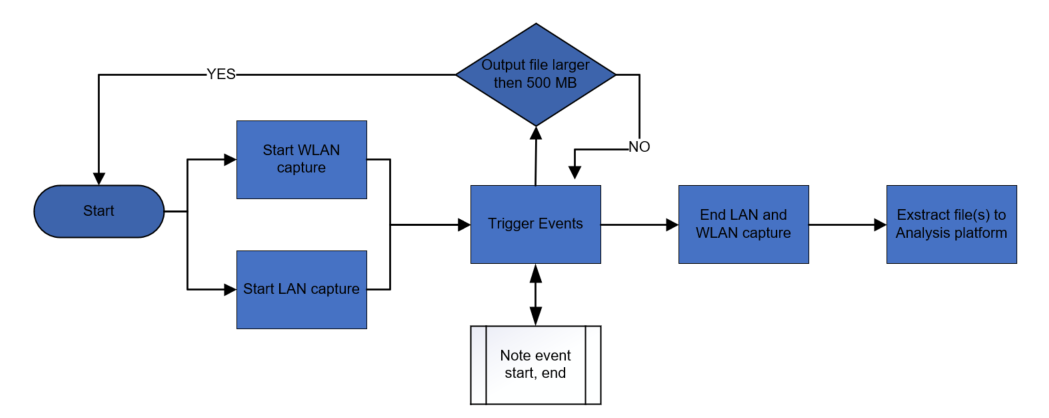
\includegraphics[width=\textwidth]{figures/Event triggering process.png}
    \caption{Capturing process}
    \label{fig:captuingprocess}
\end{figure}

\subsection{Event Selection}
This section will describe the different features that is included in the research and the overall event triggering process. Each test will be executed 10 times for each of the two environments. 10 is the number of event which is decided to be sufficient to extract signatures with human manual analysis. All events except the standby capturing will be executed 10 times in each of the two events. 


\subsubsection{Standby Traffic}
This test is executed to identify network traffic generated by the robot vacuum cleaner in a standby mode. This means that there is no interaction during the event. This will only be done in Oslo environment, due to time limitations.

\begin{itemize}
    \item \textbf{Event flow} \begin{enumerate}
                                    \item Start captuing of LAN and WLAN traffic
                                    \item Wait 14 days without any human interaction
                                    \item Stop capturing
                                \end{enumerate}
    \item \textbf{Number of events:} 1
\end{itemize}

\subsubsection{Scheduled Cleaning}
Scheduled cleaning can be configured through the application. Users can schedule a cleaning, specifying area in the smart home, time which the cleaning should start, as well as how often this should occur. 
\begin{itemize}
    \item Event flow \begin{enumerate}
                                    \item Start captuing of LAN and WLAN traffic
                                    \item Trigger cleaning event
                                    \item Note when "finish" notification is received
                                    \item Stop capturing
                                \end{enumerate}
\end{itemize}

\subsubsection{Automated Cleaning}
Irobot has features to integrate other services as triggers for events. This includes IFFF location tracker \cite{}, Agust smart lock system, ecobee termotat system, My Leviton smart home integration and MyQ garage system. In this research the IFTTT location system will be used. Cleaning is then triggered when the user's phone is x meters away from home, where x is between 100m and 1 km. This event has the same flow as scheduled cleaning event. 


\subsubsection{Application Triggered Cleaning}
In the application users can trigger cleaning. There is a predefined "clean all" option, if the user have not customized a new based on the discovered smart home map. Cleaning is triggered when the user is pressing a cleaning option in the application. This event has the same flow as scheduled cleaning event.


\subsubsection{Physical Triggered Cleaning}
The Irobot roomba i7 has a physical cleaning button on top of the vacuum cleaner. A "clean all" vent is triggered when this button is pressed. This event has the same flow as scheduled cleaning event.

\subsubsection{Application Start}
When the application is started, an information dashboard will be displayed. Users can then interact with the vacuum cleaner. 

\begin{itemize}
    \item Event flow \begin{enumerate}
                                    \item Note time
                                    \item Open the application on the smart phone
                                    \item Wait for some time
                                    \item Close application
                                    \item Note time
                                \end{enumerate}
\end{itemize}

\subsubsection{Bin Remove}
The Irobot roomba i7 has it own bin where dust is collected during clean. This can be removed if it is to be empty. The user will then have to physically remove and insert again. 

\begin{itemize}
    \item Event flow \begin{enumerate}
                                    \item Note time
                                    \item Remove the bin
                                    \item Wait  more then 30 seconds
                                    \item Insert the bin
                                    \item Note time
                                \end{enumerate}
\end{itemize}

\section{Traffic Filtering}
To make the analysis feasible for the human mind, there will be conducted some pre processing and filtering of the data. The standby traffic capture will be used for the initial processing, all traffic in this capture is either generated by the Access point or the robot vacuum cleaner. This initial processing will be done in Wireshark. Reoccurring traffic in the Standby capture can be filter out since they are not directly connected to an event that is triggered. All the identified traffic flows not relevant to events will be added to Wireshark capture filter \cite{wireshark}, and excluded from the display.

\begin{figure}[H]
    \centering
    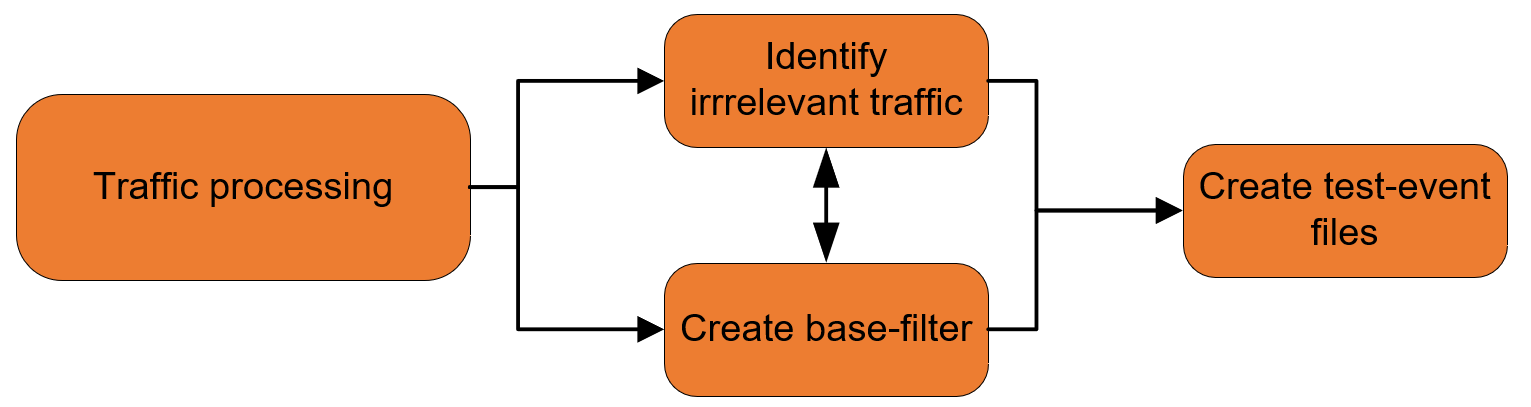
\includegraphics[width=\textwidth]{figures/TrafficProcessingProcess.png}
    \caption{Traffic processing}
    \label{fig:TrafficProcessingProcess}
\end{figure}


The Wireshark filter will be created with a series of if statements combined in a logical AND, OR and NOT equation. Each irrelevant traffic flow will be added to this combined filter. At the end of pre-processing a time filter will be added to create individual pcap files per event. This is to isolate the events in the analysis phase. This filter will use event start and end which was stored in the traffic capturing process. 

\textit{(frame.len >= " Month day, start-time") \&\& (frame.len <= "Month day, end-time")}


\section{Traffic Analysis}
The traffic analysis will be divided into three different processes, \textit{protocol and event relation, Traffic sequence identification and Overall event characteristics}. After the event signatures are identified, there will be conducted a signature comparison, to evaluate is it can uniquely identify the event.

\begin{figure}[H]
    \centering
    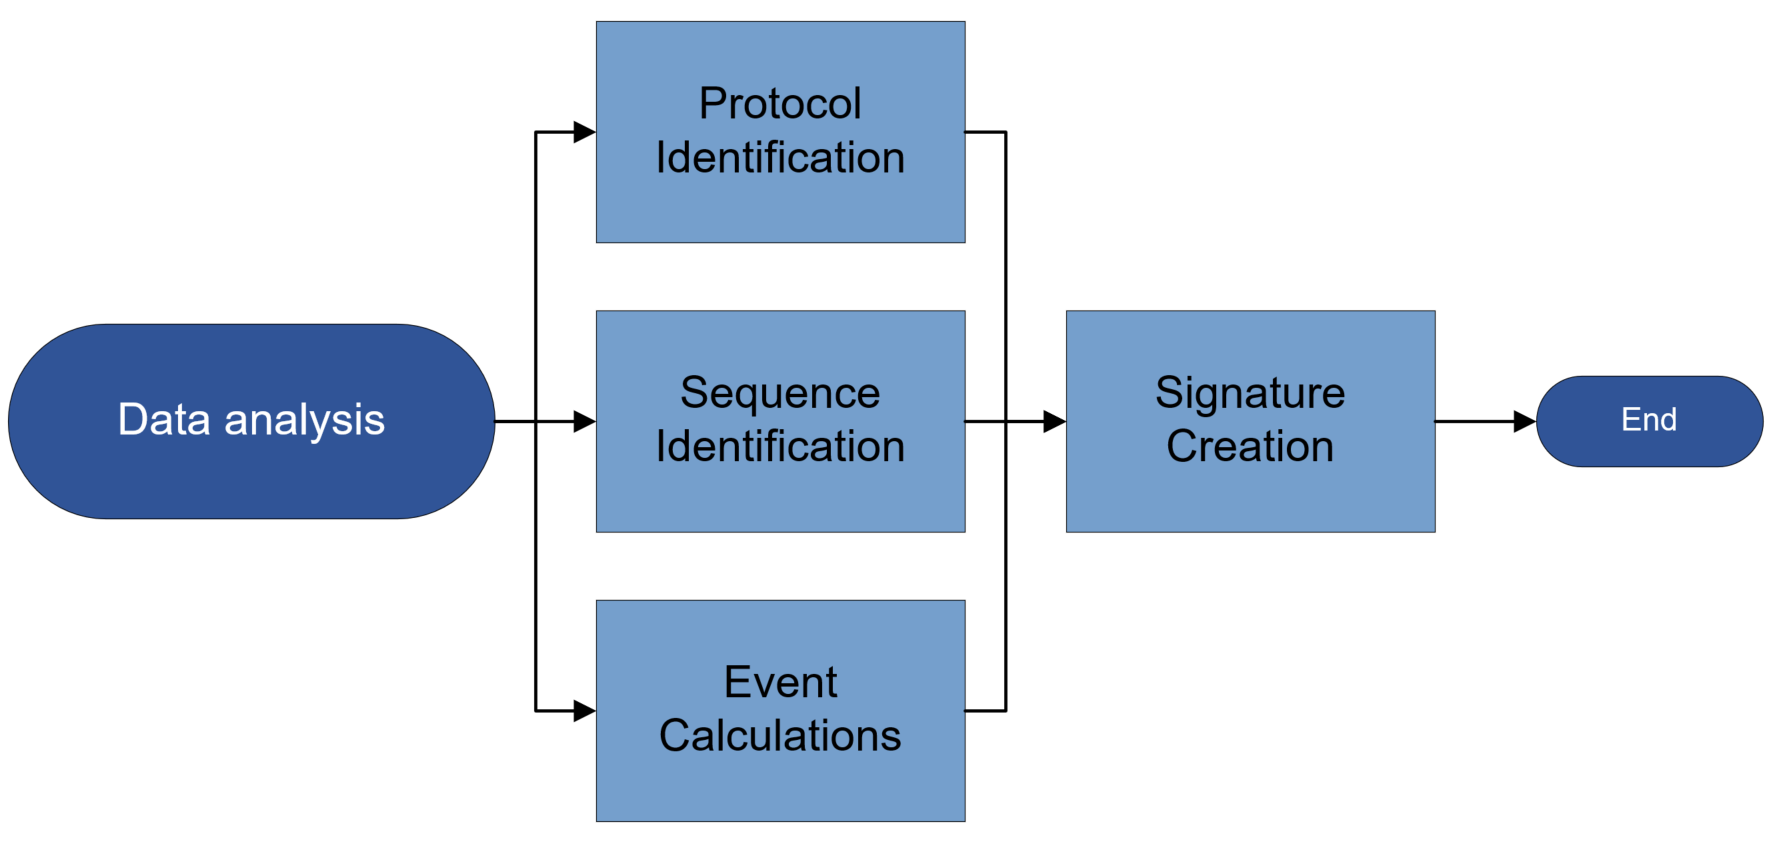
\includegraphics[width=\textwidth]{figures/TrafficAnalysisProcess.png}
    \caption{Traffic Analysis Process}
    \label{fig:TrafficAnalysisProcess}
\end{figure}

\subsection{Protocol Event Relation}
In this process Wireshark will be used to identify the different protocols in each event. Each identified protocol will then be looked at individually to see if they are relevant. 

\subsection{Traffic Sequence}
In this process the same approach as used in \cite{pingpong} will be used. For this research we will include more attributes, such as IP-address and DNS requests. The reason for this is to identify if it is possible to attribute events based the WAN traffic as well. The different sequences that will be analysed is listed below.  
\begin{itemize}
    \item Packet lengths both directions.
    \item Packet lengths with vacuum cleaner as source.
    \item Packet lengths with vacuum cleaner as destination.
\end{itemize}

\subsection{Overall Event Characteristics}
Each event has an overall characteristics, this data will be extracted and compared against the other event files. If the standard deviation between the captured events is small it will indicate that the result is persistent. Higher deviation will require more tests of a single event.
\begin{itemize}
    \item Number of packets
    \item Total bytes
    \item Different protocols
\end{itemize}

\subsection{Event Signatures}
The output from the different processes will be combined and used to create suggestion for event signatures. These signatures will be created as conditions in a python script, and applied to the different event files to see if it is possible to identify the same signature in the event files. 
If the event is identified, a confident variable is increased in value. This will be used in the overall event detection process. Below is the logic that will identify the signatures in the event files.
\begin{lstlisting}
# Python code, Signeture detection
1. def Identify_event(event_file, event_confidence_variable):
2.     event_siganture = ['siganture']
3.     if event_signature is in eventfile:
4.         event_confident_variabel =+ x
5.     else
6.         None
7.     return event_confodence_variabel
\end{lstlisting}

\section{Signature Detection and Evaluation}
All signatures with higher success rate then 80\% on the event files, will be included in the Human-learn:rule-based script. The overall logic is presented below.
\begin{lstlisting}
# Python code, Signeture detection
1. Main()
2.      #import event pcap file
3.      Capture = import(Event_file_x)
4.      #Run detection functions, and create confidence variables
5.      #eventX_confident_variable = eX_cv  
6.      e1_cv = identify_event1(Capture, event1_confodence_variable)
7.      e2_cv = identify_event2(Capture, event1_confodence_variable)
8.      e3_cv = identify_event3(Capture, event1_confodence_variable)
9.      e4_cv = identify_event4(Capture, event1_confodence_variable)
10.     e5_cv = identify_event5(Capture, event1_confodence_variable)
11.     e6_cv = identify_event6(Capture, event1_confodence_variable)
12.     #comapre event_confident_variables highest is event
13.     confident_variables = [list of all variables]
14.     for event in range(1,6)
15.          if confidentvariabels[event] is larger then last number
16.              largest = confidentvariabels[event]  
\end{lstlisting}

